%
\documentclass[times, 10pt,twocolumn]{article} 
\usepackage{latex8}
\usepackage{times}
\usepackage[portuguese]{babel}
\usepackage[utf8]{inputenc}
\usepackage{graphicx}
\usepackage{titlesec}
\titlespacing*{\section}
{0pt}{5pt}{5pt}
\titlespacing*{\subsection}
{0pt}{5pt}{5pt}
\titlespacing*{\subsubsection}
{0pt}{5pt}{5pt}

\pagestyle{empty}

\begin{document}

\title{\huge{PADI-DSTM} \\[0,1in] \textmd{Plataformas para Aplicações Distribuídas na Internet \\[0,05in] 2013-14}}

\maketitle
\thispagestyle{empty}

\begin{abstract}
O PADI-DSTM é um sistema distribuído que tem como objectivo gerir objectos alojados em diferentes servidores, com recurso a transacções. A solução apresentada segue a abordagem de TimeStamp Ordering[1], em que o master faculta timestamps únicos para cada transacção. Os vários servidores, além de alojarem e manipularem dados, também podem ser coordenadores transaccionais. O cliente sabe quem é o coordenador das suas transacções através do master. Esta solução já inclui replicação de dados, para manter a redundância dos mesmos.
\end{abstract}

\section{Introdução}


\section{Arquitectura}

\subsection{Componentes do Sistema}

\subsubsection{\textit{Master}}

Quando o cliente quer iniciar uma transacção, tem de contactar primeiro o \textit{master}, pois este é responsável por atribuir um \textit{timestamp} único a cada transacção e por escolher o que considera ser o melhor coordenador, naquele momento, para essa mesma transacção. O \textit{master} mantém ainda o registo de todos os servidores activos. 

\begin{description}

\item[Distribuição de \textit{timestamps}:]
Quando o \textit{master} recebe o pedido de início de transacção do cliente, este vai atribuir um \textit{timestamp} a essa futura transacção. O processo de geração de \textit{timestamp} consiste em consultar o seu \textit{Real Time Clock} com a precisão de microssegundos.  Este processo de entrega de \textit{timestamps} pelo \textit{master} faz com que todos os clientes criem transacções com \textit{timestamps} sequenciais. Isto é uma vantagem, uma vez que faculta uma ordem de acesso universal para o caso de diferentes transacções acederem ao mesmo objecto. A consulta do RTC não tem um peso computacional considerável, sendo esta, outra vantagem. 

\item[Escolha de coordenadores:]
Para a escolha de coordenadores o \textit{master} selecciona servidores aleatoriamente. Deste modo, algures no tempo, todos os servidores estarão a contribuir com trabalho de coordenação transaccional. Quando algum dos servidores notifica o \textit{master} que está  sobrecarregado, o \textit{master} descarta-o como opção para coordenador até que receba uma notificação do mesmo a avisar que já se encontra pronto para coordenar novamente. A vantagem desta abordagem resume-se no facto do \textit{master} não ficar sobrecarregado com trabalho de coordenação transaccional. Além disso, o \textit{master} tem sempre conhecimento quando um servidor está sobrecarregado, podendo tomar uma acção para manter o sistema equilibrado. O facto de ser o coordenador a avisar o \textit{master} caso esteja sobrecarregado, também poupa bastantes recursos, visto que não usa espera activa. O facto da escolha do coordenador ser feita de modo aleatório traz vantagens, uma vez que é mais rápida e a probabilidade do mesmo servidor ser escolhido duas vezes seguidas diminui conforme o aumento do número de servidores no sistema.

\item[Caso crítico:]
Quando todos os servidores disponíveis notificam o \textit{master} que estão sobrecarregados, então nesse caso, em específico, o \textit{master} toma a iniciativa de ser o coordenador de todas as próximas transacções até que exista pelo menos um servidor que consiga coordenar. De modo a impedir que o \textit{master} se torne \textit{bottleneck} quando está a fazer trabalho de coordenação transaccional, é imposto um valor limite de carga, que é variável conforme os teste efectuados ao sistema de modo a optimizar o mesmo. Este valor limite tem em conta o número de transacções que o \textit{master} pode estar a coordenar simultaneamente. Quando este valor é atingido, o \textit{master} rejeita pedidos de forma a manter-se funcional em relação aos pedidos sobre os quais já tem responsabilidade. 

\item[Registo de novos servidores e localização de objectos:]
O \textit{master} tem ainda como função permitir o registo de novos servidores, dando ordem de redistribuição de armazenamento se tal vier a acontecer. Além disto, o \textit{master} decide em que servidor vão ser criados os novos objectos resultantes dos pedidos dos clientes. A decisão é baseada numa fórmula que tenta dividir ao máximo, de forma equivalente, a carga total de armazenamento pelos servidores. Deste modo, o id do servidor em que vai ser criado o novo objecto é igual ao resultado de \textit{(hash(uid) mod n)}, onde n corresponde ao número de servidores e uid ao identificador numérico do objecto. Para guardar o objecto primário, sem ter em conta a réplica, a função de \textit{hash(uid)} devolve o próprio uid. Esta fórmula serve também para aceder a objectos já existentes, e nesse caso o uid corresponde ao uid do objecto a que se quer aceder.

\item[Objectos especiais:]
A fórmula anterior é válida para todos os objectos, excepto para aqueles são extremamente acedidos e residem no mesmo servidor. Estes são designados por objectos especiais. Para estes objectos é guardado no \textit{master} a sua localização real, visto que a fórmula não iria resultar neste caso. Deste modo, antes de executar a fórmula para saber onde está o objecto, verifica-se se o mesmo é um objecto especial. Isto é feito a partir da tentativa de acesso ao objecto em questão numa tabela de dispersão. Caso o acesso seja feito com sucesso (o objecto está na tabela e portanto é especial) a localização real é devolvida, caso contrário é devolvido \textit{null} e sabemos que temos que encontrar a localização a partir da fórmula genérica.

\item[Actualização dos servidores pelo \textit{master}:]
Sempre que um servidor é criado, o \textit{master} fornece-lhe a informação relativa a esta fórmula. Do mesmo modo, cada vez que um novo servidor aparece no sistema ou um objecto é considerado especial, essa informação tem que ser actualizada. Deste modo, à medida que os servidores tentam aceder à informação não actualizada é apresentado um erro. Quando os servidores se deparam com este erro, requisitam a informação ao \textit{master} e nesse momento têm acesso á informação actualizada.  A partir do momento que o servidor se regista no \textit{master},  pode também ser escolhido para ser coordenador, visto que a selecção se dá de forma aleatória entre todos os servidores.

Para facilitar o trabalho do \textit{master}, este guarda na tabela a correspondência entre o ID dos servidores e os respectivos endereços IP. Parte desta informação é enviada para o coordenador caso o mesmo faça um pedido para tal. De modo a diminuir o número de pedidos, cada coordenador tem uma \textit{cache} para este efeito.

\begin{table}
\centering
\begin{tabular}{c|c}
ID do Servidor & IP do Servidor \\\hline
0 & tcp : // 192.168.2.72:80 /Server \\
1 & tcp : // 192.168.2.73:80 /Server \\
2 & tcp : // 192.168.2.74:80 /Server \\
3 & tcp : // 192.168.2.75:80 /Server \\
\end{tabular}
\caption{\label{tab:idip}Tradução ID-IP dos servidores activos.}
\end{table}
\end{description}

\subsubsection{Servidor}

\begin{description}

\item[Gestão e manipulação de dados:]
Os servidores têm responsabilidade de se registar no \textit{master} assim que estejam activos. Têm como função guardar e alterar os objectos partilhados, deste modo podem ser vistos como um repositório. De um modo mais especifico, cada servidor, além dos objectos nativos com número de acessos considerado normal, faz ainda a distinção entre objecto especiais, objectos para replicar, objectos para migrar e objectos especiais provenientes de outros servidores. Quanto aos objectos para replicar, mantêm-se numa fila própria para o efeito até a replicação ser efectivamente concluída. Este processo de replicação só não é instantâneo quando o servidor responsável por receber a réplica \footnote{$ \textit{hash(uid+1) mod n} $} está indisponível, sendo o processo concluído quando o servidor estiver novamente disponível. Em relação aos dados para migrar, o mecanismo de fila de espera é igual, mas o servidor de destino é escolhido aleatoriamente pelo \textit{master}, entre os que estão disponíveis. 

Quando um objecto é alterado com sucesso, é da responsabilidade do servidor encaminhar essa informação até à sua réplica e também ao coordenador dessa transacção. O tipo PadInt é composto por um inteiro que corresponde ao seu valor, pelos contadores de acessos (\textit{read}/\textit{write}), pelos \textit{timestamps} das últimas versões que fizeram escritas/leituras e \textit{commits} com sucesso, e por um $\textit{enum\{TEMPORARY, DELETE, MIGRATE, NONE\}}$. Cada objecto é guardado numa tabela de dispersão criada especificamente para gerir intervalos de uids. Cada uid serve de \textit{key} para aceder ao objecto na tabela. 

\item[Marcação de dados a migrar:]
Cada vez que é feita uma escrita ou leitura a um PadInt é chamada uma função que incrementa  o número de acessos a esse objecto em específico. A métrica escolhida para contabilizar o número de acessos consiste em incrementar duas unidades no caso de se efectuar uma leitura e três no caso ser uma escrita. Quando a média do número de acessos por segundo (1000 acessos em 3 segundos) é excedida, o objecto é considerado especial pelo servidor. Note-se que a verificação do número de acessos por segundo só é feita em cada \textit{read}/\textit{write}, ou seja, o sistema só verifica quando realmente está a usar aquele objecto, minimizando assim o trabalho computacional. 

Um determinado objecto especial só é escolhido para migrar caso o número de objectos especiais existentes nesse servidor for maior que um. Quando isto acontece, o servidor notifica o \textit{master} para que este último lhe indique o endereço de um outro servidor disponível para receber o PadInt em questão. Este ultimo mecanismo nunca migra um objecto extremamente acedido para a mesma localização da sua réplica, senão iria perder-se o conceito de redundância. Isto é vantajoso na medida em que os objectos extremamente acedidos ficam distribuídos pelos diferentes servidores, permitindo assim o balanceamento de carga do sistema. Note-se ainda que o número de acessos por segundo pode ser adaptado aos mais diversos tipos de sistemas, de modo a maximizar o desempenho.

\begin{figure}[htb]
\centering
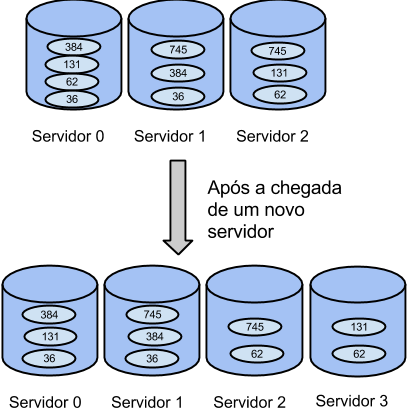
\includegraphics[width=0.5\textwidth]{migracao.png}
\caption{\label{fig:migracao}Balanceamento de carga.}
\end{figure}

\item[Versões tentativas:]
Cada coordenador gere ainda um conjunto de tentativas transaccionais (versões tentativas dos dados antes do \textit{commit}), para quando tentar fazer \textit{commit} ter essa informação disponível. Esta informação é útil porque o coordenador verifica se uma determinada transacção depende de outra para o \textit{commit} ter sucesso, e se depender, fica à espera da respectiva transacção. Assim permite-se que as transacções esperem, ao invés de abortarem devido às dependências com outras transacções. A grande vantagem desta abordagem é o paralelismo que a mesma permite, uma vez que podem executar-se bastantes transacções em cadeia, no qual o conhecimento das dependências permite que todas fazem \textit{commit} com sucesso. O facto do contexto estar nos servidores também é uma vantagem, porque permite que, se um servidor falhar, o cliente continue a executar a transacção, no servidor replicado de forma invisível, ou seja, o cliente não nota diferença no desempenho do sistema. 

\end{description}

\subsubsection{Cliente}


\subsection{Transacções e Controlo de Concorrência}

Para o controlo de concorrência é usada a abordagem \textit{TimeStamp Ordering}\cite{ex1}. Antes de iniciarem, todos os pedidos que vão constituir transações já possuem um \textit{timestamp} atribuído previamente pelo \textit{master}. Isto permite impor uma ordem de acesso aos dados e consequentemente resolver os conflitos mais cedo. Deste modo, caso uma transacção queira escrever num objecto que já foi lido por uma transacção com \textit{timestamp} superior ao seu, detecta-se logo que isto não é válido, porque não mantinha a coerência dos dados. Assim que esta anomalia é detectada, o coordenador é avisado pelo servidor e posteriormente é  feito \textit{abort} da transacção em questão. Deste modo, reduz-se a quantidade de trabalho desperdiçado, devido à detecção precoce de anomalias. O mesmo se aplica caso uma transacção queira escrever ou ler num objecto que foi escrito por uma transacção com \textit{timestamp} superior. Tome-se por excepção o caso em que uma transacção tenta escrever num objecto que já foi escrito por uma transacção com \textit{timestamp} superior, não tendo este objecto ainda ter sido lido por outra transacção. Neste caso a escrita atrasada pode ser ignorada ao invés de ser feito \textit{abort}, visto que ia ser sobreposta. Isto pode poupar recursos na medida em que se diminui o número de transacções que reiniciam.

Outra vantagem desta abordagem é que não existem \textit{deadlocks}. Além disto, quando uma transacção chega ao fim sabemos que pode fazer \textit{commit}, pois caso existisse alguma anomalia já tinha sido detectada anteriormente. Caso existam no \textit{log} versões em vias de \textit{commit} e que a transacção actual precisa de ler, a abordagem escolhida é esperar pelo \textit{commit} da outra transacção para prosseguir. Apesar da espera isto será transparente para o cliente.

Quando o cliente faz o pedido ao \textit{master} (com o método \textit{TxBegin()}) e este lhe responde com o \textit{timestamp} e o endereço IP do coordenador, o cliente  dá início à transacção, enviando o pedido, juntamente com o \textit{timestamp} para o servidor responsável por essa nova transacção. 

\begin{description}
\item[Criação de um Objecto:] Após o coordenador receber a transacção relativa ao pedido do cliente, utiliza a fórmula referida anteriormente (baseada no resto da divisão inteira) para saber em que servidor irá ser alojado aquele objecto. Em consequência, o servidor sobre o qual recaiu a responsabilidade de alojar o novo objecto é notificado sobre a criação do mesmo. Esse servidor, cria a sua versão de tentativa transaccional e caso tudo corra bem, o servidor notifica o coordenador que foi tudo feito com sucesso e que pode prosseguir com o \textit{commit}. Seguidamente o coordenador dá indicação ao servidor envolvido na transacção para guardar os dados de forma persistente (com a referência do \textit{timestamp} associado à transacção que efectuou essa criação), avisando posteriormente o cliente que a operação foi efectuada com sucesso. Caso o objecto já exista, é retornado \textit{null} e o servidor avisa o coordenador da situação, sendo que este último avisa posteriormente o cliente que a operação não foi efectuada com sucesso.

\item[Acesso a um Objecto:] O processo de leitura ou escrita é semelhante ao da criação do objecto, na medida em que também é usada a mesma fórmula para encontrar a localização do objecto. A diferença reside no facto que os acessos de leitura ou escrita seguem a metodologia do \textit{TimeStamp Ordering}\cite{ex1} referida anteriormente, comparando sempre os \textit{timestamps} da transacção actual com o \textit{timestamp} de referência (\textit{timestamp} da última transacção que manipulou o objecto com sucesso). Durante o processo, caso existam anomalias é lançada a excepção \textit{TxException} e o servidor avisa o coordenador da situação, onde este aborta a operação com o mesmo método referido anteriormente.
\end{description}

\begin{figure}[htb]
\centering
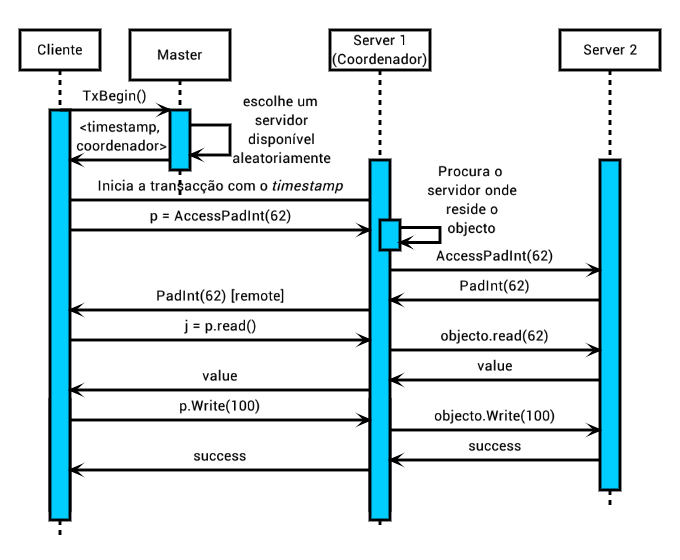
\includegraphics[width=0.5\textwidth]{transaccao.png}
\caption{\label{fig:transaccao}Diagrama transaccional.}
\end{figure}

\subsection{Tolerância a Faltas}

\subsection{Replicação}

A fórmula para encontrar o servidor em que está localizado um objecto com um dado id é \textit{"(hash(id)) mod (número de servidores)"}. Para encontrar o servidor com o objecto primário a função de dispersão retorna o id, para encontrar o servidor com a réplica a função de dispersão retorna id + j (número de objectos por bloco).
O \textit{master} contém as fórmulas mais recentes e tanto os servidores como os clientes guardam estas fórmulas em \textit{cache} no primeiro pedido efectuado ao master, para evitar pedidos remotos desnecessários.

Os clientes podem aceder aos dados de 2 maneiras:

\begin{itemize}
\item \textbf{Com replicação:} 

\begin{enumerate}
\item Cada leitura é efectuada ao servidor primário do objecto, e caso este não esteja disponível o valor é obtido do servidor secundário.

\item Cada escrita é efectuada no primário e no secundário, mas o cliente não espera pelas respostas. Caso existam mais de 2 réplicas, o cliente envia no máximo a 5 que replicam para as que faltam.
\end{enumerate}

\begin{figure}
\centering
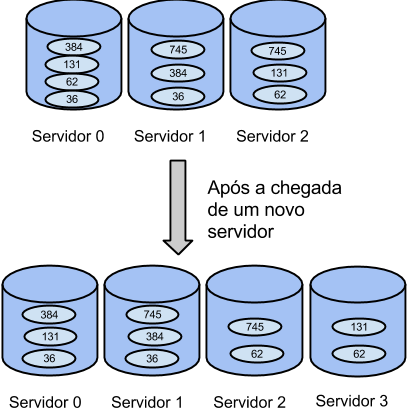
\includegraphics[width=0.4\textwidth]{migracao.png}
\caption{\label{fig:migracao}Migração dos dados face à entrada de um novo servidor.}
\end{figure}

\item \textbf{Sem replicação:}

\begin{enumerate}
\item Cada leitura é efectuada apenas no servidor responsável por guardar aquele objecto, se o servidor estiver em baixo a transacção é abortada.

\item Cada escrita é efectuada apenas no servidor responsável por guardar aquele objecto, se o servidor estiver em baixo a transacção é abortada.
\end{enumerate}
\end{itemize}

\section{Conclusão}

A solução proposta de modo a tornar o PADI-DSTM uma aplicação sequencialmente consistente reside numa abordagem de \textit{TimeStamp Ordering}[1].  Nesta solução já está contemplada a tolerância a faltas e existe distribuição de carga para que o sistema se mantenha equilibrado, tanto a nível de computação, como a nível de armazenamento. Parte das decisões tomadas para esta arquitectura (por exemplo, número máximo de transacções num coordenador), vão depender de testes ao sistema propriamente dito, pelo que numa fase inicial vão ser usados vários valores experimentais.

\nocite{ex1}
\bibliographystyle{latex8}
\bibliography{latex8}

\end{document}